\documentclass[11pt, letterpaper]{article}

% Fonts and Encoding
\usepackage[utf8]{inputenc}
\usepackage[T1]{fontenc}
\usepackage{lmodern} % High-quality Latin Modern vector font

% Math and Symbols
\usepackage{amsmath, amssymb, amsthm, amsfonts, mathrsfs, mathtools}

% Layout and Geometry
\usepackage{geometry}
\geometry{letterpaper, margin=1in}
\setlength{\parindent}{0pt}
\setlength{\parskip}{0.6em}

% Formatting and Graphics
\usepackage{graphicx, xcolor, enumitem, booktabs, array, tabularx}

% TikZ for Illustrations
\usepackage{tikz}
\usetikzlibrary{arrows.meta, positioning, shapes.geometric, calc, backgrounds, matrix}

% Clickable Links and TOC
\usepackage{hyperref}
\hypersetup{
    colorlinks=true,
    linkcolor=blue,
    filecolor=magenta,      
    urlcolor=cyan,
    pdftitle={Advanced Mathematics Topic},
}

% Theorem Environments
\newtheorem{theorem}{Theorem}[section]
\newtheorem{lemma}[theorem]{Lemma}
\newtheorem{proposition}[theorem]{Proposition}
\newtheorem{corollary}[theorem]{Corollary}
\theoremstyle{definition}
\newtheorem{definition}{Definition}[section]
\newtheorem{axiom}{Axiom}[section]
\newtheorem{example}{Example}[section]
\theoremstyle{remark}
\newtheorem{remark}{Remark}[section]

% Custom Commands (Enforced standard notation)
\newcommand{\R}{\mathbb{R}}
\newcommand{\N}{\mathbb{N}}
\newcommand{\Z}{\mathbb{Z}}
\newcommand{\Q}{\mathbb{Q}}
\newcommand{\E}{\mathbb{E}}
\newcommand{\Prob}{\mathbb{P}}
\newcommand{\F}{\mathcal{F}}
\newcommand{\Laplace}{\mathcal{L}}

\begin{document}

\title{\textbf{Mastering Impulses and the Dirac Delta Function}\\ \Large A Comprehensive Study Guide and Solution Manual}
\author{Tashfeen Omran}
\date{\today}
\maketitle

\tableofcontents
\newpage

\section{Part 1: Comprehensive Introduction, Context, and Prerequisites}

\subsection{Core Concepts}
In the study of differential equations and dynamic systems, we frequently encounter forces or inputs that act over an infinitesimally short period but deliver a finite, measurable impact. Examples include a hammer striking a mass-spring system, a lightning strike on an electrical circuit, or a concentrated point load on a structural beam. To model these mathematically, we introduce the \textbf{Dirac Delta Function}, denoted as $\delta(t)$. 

Strictly speaking, $\delta(t)$ is not a standard function but a \textit{generalized function} or \textit{distribution}. It is characterized by being zero everywhere except at the origin, where it is infinitely large, such that the total area under its curve is exactly $1$.

\subsection{Intuition and Derivation}
Imagine a force $F_n(t)$ applied over a time interval $[0, 1/n]$ with a magnitude of $n$. The total impulse (area under the curve) is $n \times (1/n) = 1$. As $n \to \infty$, the time interval shrinks to zero, and the magnitude grows to infinity, but the impulse remains constant at $1$. The Dirac delta function $\delta(t)$ is the mathematical limit of this sequence of functions $F_n(t)$. 

When we shift the function to occur at time $t = a$, we write $\delta(t-a)$. The most powerful property of the Dirac delta is its \textit{sifting property}. When multiplied by a continuous function $f(t)$ and integrated over all time, the delta function "sifts" out the value of $f(t)$ exactly at the point $t=a$.

\subsection{Historical Context and Motivation}
The delta function was formally introduced by the British theoretical physicist Paul A. M. Dirac in the 1920s to formulate quantum mechanics. Dirac needed a way to describe the density of an idealized point particle (which has mass but zero volume) and to handle continuous spectra in quantum states. Although mathematicians initially criticized it for lacking rigor, Laurent Schwartz later provided a flawless mathematical foundation for it in the 1940s through the \textit{Theory of Distributions}.

\subsection{Key Formulas}
\begin{itemize}
    \item \textbf{Definition:} $\delta(t-a) = 0$ for $t \neq a$, and $\int_{-\infty}^{\infty} \delta(t-a) \, dt = 1$.
    \item \textbf{Sifting Property:} $\int_{-\infty}^{\infty} f(t)\delta(t-a) \, dt = f(a)$.
    \item \textbf{Laplace Transform:} $\Laplace\{\delta(t-a)\}(s) = e^{-as}$ for $a \geq 0$.
    \item \textbf{Relationship to Unit Step:} $\delta(t-a) = \frac{d}{dt} u(t-a)$, where $u(t)$ is the Heaviside step function.
\end{itemize}

\subsection{Prerequisites}
To master this topic, you must be proficient in:
\begin{enumerate}
    \item \textbf{Laplace Transforms:} Computing transforms of standard functions and using the First and Second Translation Theorems.
    \item \textbf{Partial Fraction Decomposition:} Breaking down complex rational functions in the $s$-domain.
    \item \textbf{Initial Value Problems (IVPs):} Solving linear ODEs using the Laplace transform method.
\end{enumerate}

\newpage
\section{Part 2: Detailed Homework Solutions}

\subsection{Evaluating Integrals (Problems 1--6)}

\textbf{Problem 1:} Evaluate $\int_{-\infty}^{\infty} (t^2 - 1)\delta(t) \, dt$.
\\[4pt]
\textbf{Solution:} Using the sifting property $\int_{-\infty}^{\infty} f(t)\delta(t-a) \, dt = f(a)$ with $a=0$ and $f(t) = t^2 - 1$:
\[ \int_{-\infty}^{\infty} (t^2 - 1)\delta(t) \, dt = f(0) = 0^2 - 1 = -1 \]

\textbf{Problem 2:} Evaluate $\int_{-\infty}^{\infty} e^{3t}\delta(t) \, dt$.
\\[4pt]
\textbf{Solution:} Here, $f(t) = e^{3t}$ and $a=0$.
\[ \int_{-\infty}^{\infty} e^{3t}\delta(t) \, dt = e^{3(0)} = 1 \]

\textbf{Problem 3:} Evaluate $\int_{-\infty}^{\infty} (\sin 3t)\delta\left(t - \frac{\pi}{2}\right) \, dt$.
\\[4pt]
\textbf{Solution:} Here, $f(t) = \sin(3t)$ and $a = \frac{\pi}{2}$.
\[ \int_{-\infty}^{\infty} (\sin 3t)\delta\left(t - \frac{\pi}{2}\right) \, dt = \sin\left(3 \cdot \frac{\pi}{2}\right) = \sin\left(\frac{3\pi}{2}\right) = -1 \]

\textbf{Problem 4:} Evaluate $\int_{-\infty}^{\infty} e^{-2t}\delta(t + 1) \, dt$.
\\[4pt]
\textbf{Solution:} Here, $f(t) = e^{-2t}$ and $a = -1$.
\[ \int_{-\infty}^{\infty} e^{-2t}\delta(t + 1) \, dt = e^{-2(-1)} = e^2 \]

\textbf{Problem 5:} Evaluate $\int_{0}^{\infty} e^{-2t}\delta(t - 1) \, dt$.
\\[4pt]
\textbf{Solution:} The integration bounds $[0, \infty)$ contain the impulse at $t=1$. Thus, the sifting property applies.
\[ \int_{0}^{\infty} e^{-2t}\delta(t - 1) \, dt = e^{-2(1)} = e^{-2} \]

\textbf{Problem 6:} Evaluate $\int_{-1}^{1} (\cos 2t)\delta(t) \, dt$.
\\[4pt]
\textbf{Solution:} The interval $[-1, 1]$ contains $t=0$.
\[ \int_{-1}^{1} (\cos 2t)\delta(t) \, dt = \cos(2 \cdot 0) = 1 \]

\subsection{Laplace Transforms of Generalized Functions (Problems 7--12)}

\textbf{Problem 7:} Determine the Laplace transform of $\delta(t - 1) - \delta(t - 3)$.
\\[4pt]
\textbf{Solution:} Using linearity and $\Laplace\{\delta(t-a)\} = e^{-as}$:
\[ \Laplace\{\delta(t - 1) - \delta(t - 3)\} = e^{-s} - e^{-3s} \]

\textbf{Problem 8:} Determine the Laplace transform of $3\delta(t - 1)$.
\\[4pt]
\textbf{Solution:} 
\[ \Laplace\{3\delta(t - 1)\} = 3e^{-s} \]

\textbf{Problem 9:} Determine the Laplace transform of $t\delta(t - 1)$.
\\[4pt]
\textbf{Solution:} Since $f(t)\delta(t-a) = f(a)\delta(t-a)$, we have $t\delta(t-1) = 1 \cdot \delta(t-1)$.
\[ \Laplace\{t\delta(t - 1)\} = \Laplace\{\delta(t-1)\} = e^{-s} \]

\textbf{Problem 10:} Determine the Laplace transform of $t^3\delta(t - 3)$.
\\[4pt]
\textbf{Solution:} $t^3\delta(t-3) = 3^3\delta(t-3) = 27\delta(t-3)$.
\[ \Laplace\{27\delta(t - 3)\} = 27e^{-3s} \]

\textbf{Problem 11:} Determine the Laplace transform of $\delta(t - \pi)\sin t$.
\\[4pt]
\textbf{Solution:} $\delta(t-\pi)\sin t = \sin(\pi)\delta(t-\pi) = 0 \cdot \delta(t-\pi) = 0$.
\[ \Laplace\{0\} = 0 \]

\textbf{Problem 12:} Determine the Laplace transform of $e^t\delta(t - 3)$.
\\[4pt]
\textbf{Solution:} $e^t\delta(t-3) = e^3\delta(t-3)$.
\[ \Laplace\{e^3\delta(t - 3)\} = e^3 e^{-3s} = e^{3-3s} \]

\subsection{Solving Symbolic Initial Value Problems (Problems 13--20)}

\textbf{Problem 13:} Solve $w'' + w = \delta(t - \pi); \quad w(0) = 0, \quad w'(0) = 0$.
\\[4pt]
\textbf{Solution:} Take the Laplace transform of both sides:
\[ s^2 W(s) + W(s) = e^{-\pi s} \implies W(s)(s^2 + 1) = e^{-\pi s} \implies W(s) = \frac{e^{-\pi s}}{s^2 + 1} \]
Using the Second Translation Theorem, $\Laplace^{-1}\{e^{-as}F(s)\} = f(t-a)u(t-a)$:
\[ w(t) = \sin(t - \pi)u(t - \pi) = -\sin(t)u(t - \pi) \]

\textbf{Problem 14:} Solve $y'' + 2y' + 2y = \delta(t - \pi); \quad y(0) = 1, \quad y'(0) = 1$.
\\[4pt]
\textbf{Solution:} Take the Laplace transform:
\[ [s^2 Y(s) - s(1) - 1] + 2[sY(s) - 1] + 2Y(s) = e^{-\pi s} \]
\[ Y(s)(s^2 + 2s + 2) - s - 3 = e^{-\pi s} \implies Y(s) = \frac{s + 3}{s^2 + 2s + 2} + \frac{e^{-\pi s}}{s^2 + 2s + 2} \]
Complete the square in the denominator: $s^2 + 2s + 2 = (s+1)^2 + 1$.
\[ Y(s) = \frac{s + 1}{(s+1)^2 + 1} + \frac{2}{(s+1)^2 + 1} + \frac{e^{-\pi s}}{(s+1)^2 + 1} \]
Taking the inverse Laplace transform:
\[ y(t) = e^{-t}\cos t + 2e^{-t}\sin t + e^{-(t-\pi)}\sin(t-\pi)u(t-\pi) \]
Simplifying using $\sin(t-\pi) = -\sin t$:
\[ y(t) = e^{-t}(\cos t + 2\sin t) - e^{\pi-t}\sin(t)u(t-\pi) \]

\textbf{Problem 15:} Solve $y'' + 2y' - 3y = \delta(t - 1) - \delta(t - 2); \quad y(0) = 2, \quad y'(0) = -2$.
\\[4pt]
\textbf{Solution:} Take the Laplace transform:
\[ [s^2 Y - 2s - (-2)] + 2[sY - 2] - 3Y = e^{-s} - e^{-2s} \]
\[ Y(s)(s^2 + 2s - 3) - 2s - 2 = e^{-s} - e^{-2s} \implies Y(s) = \frac{2s + 2}{(s-1)(s+3)} + \frac{e^{-s} - e^{-2s}}{(s-1)(s+3)} \]
Partial fraction decomposition for the first term:
\[ \frac{2s + 2}{(s-1)(s+3)} = \frac{1}{s-1} + \frac{1}{s+3} \]
For the second term:
\[ \frac{1}{(s-1)(s+3)} = \frac{1/4}{s-1} - \frac{1/4}{s+3} \]
Inverse transform:
\[ y(t) = e^t + e^{-3t} + \frac{1}{4}\left(e^{t-1} - e^{-3(t-1)}\right)u(t-1) - \frac{1}{4}\left(e^{t-2} - e^{-3(t-2)}\right)u(t-2) \]

\textbf{Problem 16:} Solve $y'' - 2y' - 3y = 2\delta(t - 1) - \delta(t - 3); \quad y(0) = 2, \quad y'(0) = 2$.
\\[4pt]
\textbf{Solution:} Take the Laplace transform:
\[ [s^2 Y - 2s - 2] - 2[sY - 2] - 3Y = 2e^{-s} - e^{-3s} \]
\[ Y(s)(s^2 - 2s - 3) - 2s + 2 = 2e^{-s} - e^{-3s} \implies Y(s) = \frac{2s - 2}{(s-3)(s+1)} + \frac{2e^{-s} - e^{-3s}}{(s-3)(s+1)} \]
Partial fractions:
\[ \frac{2s - 2}{(s-3)(s+1)} = \frac{1}{s-3} + \frac{1}{s+1}, \quad \frac{1}{(s-3)(s+1)} = \frac{1/4}{s-3} - \frac{1/4}{s+1} \]
Inverse transform:
\[ y(t) = e^{3t} + e^{-t} + \frac{1}{2}\left(e^{3(t-1)} - e^{-(t-1)}\right)u(t-1) - \frac{1}{4}\left(e^{3(t-3)} - e^{-(t-3)}\right)u(t-3) \]

\textbf{Problem 17:} Solve $y'' - y = 4\delta(t - 2) + t^2; \quad y(0) = 0, \quad y'(0) = 2$.
\\[4pt]
\textbf{Solution:} Take the Laplace transform:
\[ [s^2 Y - 2] - Y = 4e^{-2s} + \frac{2}{s^3} \implies Y(s)(s^2 - 1) = 2 + 4e^{-2s} + \frac{2}{s^3} \]
\[ Y(s) = \frac{2}{s^2 - 1} + \frac{4e^{-2s}}{s^2 - 1} + \frac{2}{s^3(s^2 - 1)} \]
We decompose the last term algebraically:
\[ \frac{2}{s^3(s^2 - 1)} = \frac{2s^2 - 2(s^2 - 1)}{s^3(s^2 - 1)} = \frac{2}{s(s^2 - 1)} - \frac{2}{s^3} = \frac{2s^2 - 2(s^2 - 1)}{s(s^2 - 1)} - \frac{2}{s^3} = \frac{2s}{s^2 - 1} - \frac{2}{s} - \frac{2}{s^3} \]
Substitute this back into $Y(s)$:
\[ Y(s) = \frac{2}{s^2 - 1} + \frac{4e^{-2s}}{s^2 - 1} + \frac{2s}{s^2 - 1} - \frac{2}{s} - \frac{2}{s^3} \]
Inverse transform:
\[ y(t) = 2\sinh t + 4\sinh(t-2)u(t-2) + 2\cosh t - 2 - t^2 \]

\textbf{Problem 18:} Solve $y'' - y' - 2y = 3\delta(t - 1) + e^t; \quad y(0) = 0, \quad y'(0) = 3$.
\\[4pt]
\textbf{Solution:} Take the Laplace transform:
\[ [s^2 Y - 3] - sY - 2Y = 3e^{-s} + \frac{1}{s-1} \implies Y(s)(s-2)(s+1) = 3 + \frac{1}{s-1} + 3e^{-s} \]
\[ Y(s) = \frac{3}{(s-2)(s+1)} + \frac{1}{(s-1)(s-2)(s+1)} + \frac{3e^{-s}}{(s-2)(s+1)} \]
Partial fractions:
\[ \frac{3}{(s-2)(s+1)} = \frac{1}{s-2} - \frac{1}{s+1} \]
\[ \frac{1}{(s-1)(s-2)(s+1)} = -\frac{1/2}{s-1} + \frac{1/3}{s-2} + \frac{1/6}{s+1} \]
Combining the non-delayed terms:
\[ Y(s) = \frac{4/3}{s-2} - \frac{5/6}{s+1} - \frac{1/2}{s-1} + e^{-s}\left(\frac{1}{s-2} - \frac{1}{s+1}\right) \]
Inverse transform:
\[ y(t) = \frac{4}{3}e^{2t} - \frac{5}{6}e^{-t} - \frac{1}{2}e^t + \left(e^{2(t-1)} - e^{-(t-1)}\right)u(t-1) \]

\textbf{Problem 19:} Solve $w'' + 6w' + 5w = e^t\delta(t - 1); \quad w(0) = 0, \quad w'(0) = 4$.
\\[4pt]
\textbf{Solution:} First, simplify the forcing function: $e^t\delta(t-1) = e^1\delta(t-1) = e\delta(t-1)$.
\[ [s^2 W - 4] + 6sW + 5W = e \cdot e^{-s} \implies W(s)(s+1)(s+5) = 4 + e^{1-s} \]
\[ W(s) = \frac{4}{(s+1)(s+5)} + \frac{e^{1-s}}{(s+1)(s+5)} \]
Partial fractions: $\frac{1}{(s+1)(s+5)} = \frac{1/4}{s+1} - \frac{1/4}{s+5}$.
\[ w(t) = e^{-t} - e^{-5t} + \frac{e}{4}\left(e^{-(t-1)} - e^{-5(t-1)}\right)u(t-1) \]

\textbf{Problem 20:} Solve $y'' + 5y' + 6y = e^{-t}\delta(t - 2); \quad y(0) = 2, \quad y'(0) = -5$.
\\[4pt]
\textbf{Solution:} Simplify forcing function: $e^{-t}\delta(t-2) = e^{-2}\delta(t-2)$.
\[ [s^2 Y - 2s + 5] + 5[sY - 2] + 6Y = e^{-2}e^{-2s} \implies Y(s)(s+2)(s+3) = 2s + 5 + e^{-2(s+1)} \]
\[ Y(s) = \frac{2s + 5}{(s+2)(s+3)} + \frac{e^{-2(s+1)}}{(s+2)(s+3)} \]
Partial fractions: $\frac{2s+5}{(s+2)(s+3)} = \frac{1}{s+2} + \frac{1}{s+3}$ and $\frac{1}{(s+2)(s+3)} = \frac{1}{s+2} - \frac{1}{s+3}$.
\[ y(t) = e^{-2t} + e^{-3t} + e^{-2}\left(e^{-2(t-2)} - e^{-3(t-2)}\right)u(t-2) \]

\subsection{Symbolic IVPs and Graphing (Problems 21--24)}

\textbf{Problem 21:} $y'' + y = \delta(t - 2\pi); \quad y(0) = 0, \quad y'(0) = 1$.
\\[4pt]
\textbf{Solution:} $Y(s) = \frac{1}{s^2+1} + \frac{e^{-2\pi s}}{s^2+1} \implies y(t) = \sin t + \sin(t-2\pi)u(t-2\pi) = \sin t + \sin t \, u(t-2\pi)$.

\textbf{Problem 22:} $y'' + y = \delta(t - \pi/2); \quad y(0) = 0, \quad y'(0) = 1$.
\\[4pt]
\textbf{Solution:} $Y(s) = \frac{1}{s^2+1} + \frac{e^{-\pi s/2}}{s^2+1} \implies y(t) = \sin t + \sin(t-\pi/2)u(t-\pi/2) = \sin t - \cos t \, u(t-\pi/2)$.

\textbf{Problem 23:} $y'' + y = -\delta(t - \pi) + \delta(t - 2\pi); \quad y(0) = 0, \quad y'(0) = 1$.
\\[4pt]
\textbf{Solution:} $Y(s) = \frac{1}{s^2+1} - \frac{e^{-\pi s}}{s^2+1} + \frac{e^{-2\pi s}}{s^2+1} \implies y(t) = \sin t + \sin t \, u(t-\pi) + \sin t \, u(t-2\pi)$.

\textbf{Problem 24:} $y'' + y = \delta(t - \pi) - \delta(t - 2\pi); \quad y(0) = 0, \quad y'(0) = 1$.
\\[4pt]
\textbf{Solution:} $Y(s) = \frac{1}{s^2+1} + \frac{e^{-\pi s}}{s^2+1} - \frac{e^{-2\pi s}}{s^2+1} \implies y(t) = \sin t - \sin t \, u(t-\pi) - \sin t \, u(t-2\pi)$.

\vspace{1em}
\begin{center}
\begin{tikzpicture}[scale=0.85]
    \fill[white] (-1,-1) rectangle (16, 10);
    
    % Problem 21
    \begin{scope}[shift={(0,6)}]
        \draw[thick, ->] (0,0) -- (7,0) node[right] {$t$};
        \draw[thick, ->] (0,-2.5) -- (0,2.5) node[above] {$y(t)$};
        \draw[ultra thick, blue!80!black, domain=0:2*pi, samples=100] plot (\x, {sin(\x r)});
        \draw[ultra thick, blue!80!black, domain=2*pi:3*pi, samples=50] plot (\x, {2*sin(\x r)});
        \draw[thick] (2*pi, 0.1) -- (2*pi, -0.1) node[below] {$2\pi$};
        \node[align=left, anchor=west, inner sep=6pt] at (7.5, 1) {\textbf{Problem 21}\\[4pt] $\displaystyle y(t) = \sin t + \sin t \, u(t-2\pi)$};
    \end{scope}

    % Problem 22
    \begin{scope}[shift={(0,0)}]
        \draw[thick, ->] (0,0) -- (7,0) node[right] {$t$};
        \draw[thick, ->] (0,-2.5) -- (0,2.5) node[above] {$y(t)$};
        \draw[ultra thick, blue!80!black, domain=0:pi/2, samples=50] plot (\x, {sin(\x r)});
        \draw[ultra thick, blue!80!black, domain=pi/2:3*pi, samples=100] plot (\x, {sin(\x r) - cos(\x r)});
        \draw[thick] (pi/2, 0.1) -- (pi/2, -0.1) node[above left] {$\pi/2$};
        \node[align=left, anchor=west, inner sep=6pt] at (7.5, 1) {\textbf{Problem 22}\\[4pt] $\displaystyle y(t) = \sin t - \cos t \, u(t-\pi/2)$};
    \end{scope}
\end{tikzpicture}

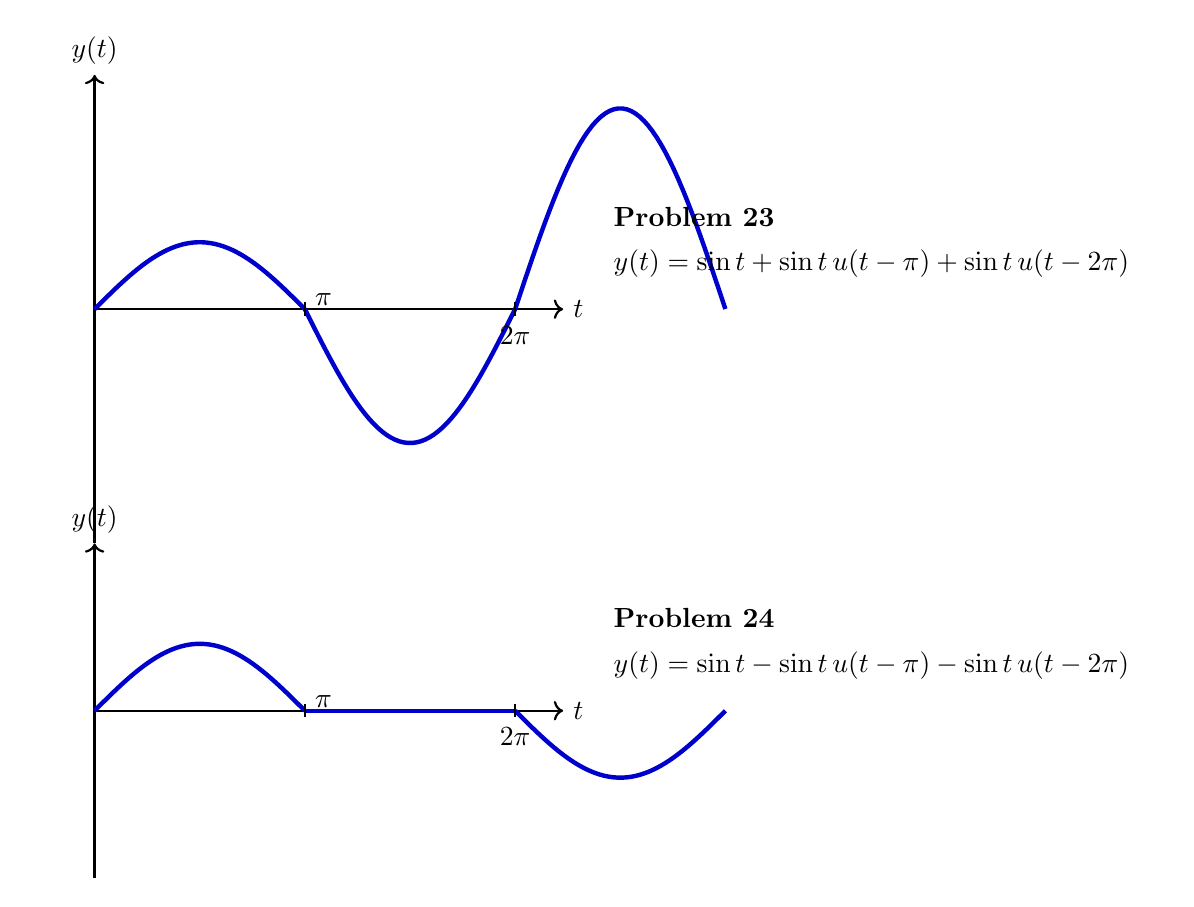
\begin{tikzpicture}[scale=0.85]
    \fill[white] (-1,-1) rectangle (16, 10);
    
    % Problem 23
    \begin{scope}[shift={(0,6)}]
        \draw[thick, ->] (0,0) -- (7,0) node[right] {$t$};
        \draw[thick, ->] (0,-3.5) -- (0,3.5) node[above] {$y(t)$};
        \draw[ultra thick, blue!80!black, domain=0:pi, samples=50] plot (\x, {sin(\x r)});
        \draw[ultra thick, blue!80!black, domain=pi:2*pi, samples=50] plot (\x, {2*sin(\x r)});
        \draw[ultra thick, blue!80!black, domain=2*pi:3*pi, samples=50] plot (\x, {3*sin(\x r)});
        \draw[thick] (pi, 0.1) -- (pi, -0.1) node[above right] {$\pi$};
        \draw[thick] (2*pi, 0.1) -- (2*pi, -0.1) node[below] {$2\pi$};
        \node[align=left, anchor=west, inner sep=6pt] at (7.5, 1) {\textbf{Problem 23}\\[4pt] $\displaystyle y(t) = \sin t + \sin t \, u(t-\pi) + \sin t \, u(t-2\pi)$};
    \end{scope}

    % Problem 24
    \begin{scope}[shift={(0,0)}]
        \draw[thick, ->] (0,0) -- (7,0) node[right] {$t$};
        \draw[thick, ->] (0,-2.5) -- (0,2.5) node[above] {$y(t)$};
        \draw[ultra thick, blue!80!black, domain=0:pi, samples=50] plot (\x, {sin(\x r)});
        \draw[ultra thick, blue!80!black, domain=pi:2*pi, samples=50] plot (\x, {0});
        \draw[ultra thick, blue!80!black, domain=2*pi:3*pi, samples=50] plot (\x, {-sin(\x r)});
        \draw[thick] (pi, 0.1) -- (pi, -0.1) node[above right] {$\pi$};
        \draw[thick] (2*pi, 0.1) -- (2*pi, -0.1) node[below] {$2\pi$};
        \node[align=left, anchor=west, inner sep=6pt] at (7.5, 1) {\textbf{Problem 24}\\[4pt] $\displaystyle y(t) = \sin t - \sin t \, u(t-\pi) - \sin t \, u(t-2\pi)$};
    \end{scope}
\end{tikzpicture}
\end{center}

\subsection{Impulse Response Functions (Problems 25--28)}
The impulse response $h(t)$ is the solution to $ay''+by'+cy = \delta(t)$ with zero initial conditions. Thus, $H(s) = \frac{1}{as^2+bs+c}$.

\textbf{Problem 25:} $y'' + 4y' + 8y = g(t)$.
\\[4pt]
\textbf{Solution:} $H(s) = \frac{1}{s^2+4s+8} = \frac{1}{(s+2)^2+4} \implies h(t) = \frac{1}{2}e^{-2t}\sin(2t)$.

\textbf{Problem 26:} $y'' - 6y' + 13y = g(t)$.
\\[4pt]
\textbf{Solution:} $H(s) = \frac{1}{s^2-6s+13} = \frac{1}{(s-3)^2+4} \implies h(t) = \frac{1}{2}e^{3t}\sin(2t)$.

\textbf{Problem 27:} $y'' - 2y' + 5y = g(t)$.
\\[4pt]
\textbf{Solution:} $H(s) = \frac{1}{s^2-2s+5} = \frac{1}{(s-1)^2+4} \implies h(t) = \frac{1}{2}e^{t}\sin(2t)$.

\textbf{Problem 28:} $y'' - y = g(t)$.
\\[4pt]
\textbf{Solution:} $H(s) = \frac{1}{s^2-1} = \frac{1}{2}\left(\frac{1}{s-1} - \frac{1}{s+1}\right) \implies h(t) = \frac{1}{2}(e^t - e^{-t}) = \sinh(t)$.

\subsection{Applied and Theoretical Problems (Problems 29--35)}

\textbf{Problem 29:} Solve $x'' + 9x = -3\delta(t - \pi/2); \quad x(0) = 1, \quad x'(0) = 0$. What happens to the mass after it is struck?
\\[4pt]
\textbf{Solution:} 
\[ s^2 X - s + 9X = -3e^{-\pi s/2} \implies X(s) = \frac{s}{s^2+9} - \frac{3e^{-\pi s/2}}{s^2+9} \]
\[ x(t) = \cos(3t) - \sin\left(3\left(t - \frac{\pi}{2}\right)\right)u\left(t - \frac{\pi}{2}\right) = \cos(3t) - \sin\left(3t - \frac{3\pi}{2}\right)u\left(t - \frac{\pi}{2}\right) \]
Since $\sin(3t - 3\pi/2) = \cos(3t)$, we have $x(t) = \cos(3t) - \cos(3t)u(t - \pi/2)$. 
\textbf{Conclusion:} For $t > \pi/2$, $x(t) = 0$. The impulse perfectly cancels the momentum, bringing the mass to a complete and permanent stop.

\textbf{Problem 30:} Solve $y'' + y = \sum_{k=1}^{\infty} \delta(t - 2k\pi); \quad y(0) = 0, \quad y'(0) = 0$. Explain why soldiers are told not to march in cadence.
\\[4pt]
\textbf{Solution:} 
\[ Y(s) = \sum_{k=1}^{\infty} \frac{e^{-2k\pi s}}{s^2+1} \implies y(t) = \sum_{k=1}^{\infty} \sin(t - 2k\pi)u(t - 2k\pi) = \sum_{k=1}^{\infty} \sin(t)u(t - 2k\pi) \]
\textbf{Conclusion:} Every time $t$ crosses a multiple of $2\pi$, another $\sin(t)$ term is added. The amplitude of the oscillation grows linearly without bound (resonance). This models why soldiers marching in cadence can cause a bridge to collapse.

\textbf{Problem 31 \& 32:} Show that a linear system $ay''+by'+cy=g(t)$ is stable (bounded impulse response) iff the real parts of the roots of $ar^2+br+c=0$ are $\le 0$, and asymptotically stable ($h(t) \to 0$) iff the real parts are strictly $< 0$.
\\[4pt]
\textbf{Solution:} The impulse response $h(t)$ is the inverse Laplace transform of $H(s) = \frac{1}{as^2+bs+c}$. The roots of the denominator dictate the form of $h(t)$. If roots $r_1, r_2$ are distinct, $h(t) = A e^{r_1 t} + B e^{r_2 t}$. If they are complex $r = \alpha \pm i\beta$, $h(t) = A e^{\alpha t}\sin(\beta t)$. 
For $h(t)$ to remain bounded as $t \to \infty$, the exponential terms must not grow, which requires the real part $\alpha \le 0$. For $h(t) \to 0$ (asymptotic stability), the exponential terms must strictly decay, requiring $\alpha < 0$.

\textbf{Problem 33:} Verify $\int_{-\infty}^{\infty} f(t)\delta(t) \, dt = f(0)$ using the Mean Value Theorem for Integrals.
\\[4pt]
\textbf{Solution:} Let $\delta(t)$ be approximated by a pulse $F_n(t)$ of width $1/n$ and height $n$ centered at $0$. By the MVT for integrals, $\int_{-1/(2n)}^{1/(2n)} f(t)F_n(t) \, dt = f(c_n) \int_{-1/(2n)}^{1/(2n)} F_n(t) \, dt = f(c_n) \cdot 1$, where $c_n \in [-1/(2n), 1/(2n)]$. As $n \to \infty$, the interval shrinks to $0$, forcing $c_n \to 0$. Since $f$ is continuous, $f(c_n) \to f(0)$.

\textbf{Problem 34:} Show $\int_{-\infty}^{\infty} f(t)\delta'(t) \, dt = -f'(0)$.
\\[4pt]
\textbf{Solution:} Use integration by parts. Let $u = f(t)$ and $dv = \delta'(t) \, dt$. Then $du = f'(t) \, dt$ and $v = \delta(t)$.
\[ \int_{-\infty}^{\infty} f(t)\delta'(t) \, dt = \left[ f(t)\delta(t) \right]_{-\infty}^{\infty} - \int_{-\infty}^{\infty} f'(t)\delta(t) \, dt \]
Since $\delta(t) = 0$ at $\pm \infty$, the boundary term vanishes. The remaining integral is evaluated using the sifting property: $-f'(0)$.

\textbf{Problem 35:} Solve $EI y^{(4)}(x) = L\delta(x - \lambda)$ with $y(0) = y'(0) = y''(2\lambda) = y'''(2\lambda) = 0$.
\\[4pt]
\textbf{Solution:} Take the Laplace transform with respect to $x$. Let $y''(0) = A$ and $y'''(0) = B$.
\[ s^4 Y(s) - s^3(0) - s^2(0) - sA - B = \frac{L}{EI}e^{-\lambda s} \implies Y(s) = \frac{A}{s^3} + \frac{B}{s^4} + \frac{L}{EI s^4}e^{-\lambda s} \]
Inverse transform:
\[ y(x) = \frac{A}{2}x^2 + \frac{B}{6}x^3 + \frac{L}{6EI}(x - \lambda)^3 u(x - \lambda) \]
Differentiate to apply boundary conditions at $x = 2\lambda$:
\[ y''(x) = A + Bx + \frac{L}{EI}(x - \lambda)u(x - \lambda) \implies y''(2\lambda) = A + 2B\lambda + \frac{L\lambda}{EI} = 0 \]
\[ y'''(x) = B + \frac{L}{EI}u(x - \lambda) \implies y'''(2\lambda) = B + \frac{L}{EI} = 0 \implies B = -\frac{L}{EI} \]
Substitute $B$ into the $y''$ equation: $A - \frac{2L\lambda}{EI} + \frac{L\lambda}{EI} = 0 \implies A = \frac{L\lambda}{EI}$.
Final solution:
\[ y(x) = \frac{L\lambda}{2EI}x^2 - \frac{L}{6EI}x^3 + \frac{L}{6EI}(x - \lambda)^3 u(x - \lambda) \]

\newpage
\section{Part 3: In-Depth Analysis of Problems and Techniques}

\subsection{A) Problem Types and General Approach}
\begin{itemize}
    \item \textbf{Integral Evaluation (1-6):} These test the fundamental sifting property. The strategy is to identify the point $t=a$ where the impulse occurs, check if $a$ is within the integration bounds, and evaluate the multiplied function $f(a)$.
    \item \textbf{Laplace Transforms of Impulses (7-12):} These require applying the rule $\Laplace\{\delta(t-a)\} = e^{-as}$. If the impulse is multiplied by a function $f(t)$, you must first simplify $f(t)\delta(t-a)$ to $f(a)\delta(t-a)$ before transforming.
    \item \textbf{Symbolic IVPs (13-24):} The core application. Strategy: Take the Laplace transform, isolate $Y(s)$, perform partial fraction decomposition, and use the Second Translation Theorem to find $y(t)$.
    \item \textbf{Theoretical Proofs \& Modeling (29-35):} These problems connect the abstract math to physical reality (e.g., stopping a mass, resonance, beam deflection). The strategy involves setting up the IVP/BVP and interpreting the piecewise nature of the solution.
\end{itemize}

\subsection{B) Key Algebraic and Calculus Manipulations}
\begin{itemize}
    \item \textbf{Pre-Transform Simplification:} In Problem 19, simplifying $e^t\delta(t-1)$ to $e^1\delta(t-1)$ before taking the transform is crucial. Attempting to use convolution or shift theorems here would lead to a dead end.
    \item \textbf{Completing the Square:} Used in Problems 14, 25, 26, and 27. When the denominator $as^2+bs+c$ has complex roots, rewriting it as $(s-h)^2 + k^2$ allows the use of the $e^{at}\sin(kt)$ inverse transform formulas.
    \item \textbf{Advanced Partial Fractions:} In Problem 17, decomposing $\frac{2}{s^3(s^2-1)}$ required recognizing that $\frac{1}{s^2-1} - \frac{1}{s^2} = \frac{1}{s^2(s^2-1)}$. Algebraic agility here prevents solving massive $5 \times 5$ systems of equations.
\end{itemize}

\newpage
\section{Part 4: "Cheatsheet" and Tips for Success}

\renewcommand{\arraystretch}{1.5}
\begin{tabularx}{\textwidth}{l >{$\displaystyle}c<{$} X}
\toprule
\textbf{Concept} & \text{\textbf{Formula}} & \textbf{Description} \\
\midrule
Sifting Property & \int_{-\infty}^{\infty} f(t)\delta(t-a) \, dt = f(a) & Extracts the value of $f(t)$ at the exact moment the impulse fires. \\
\addlinespace[4pt]
Laplace Transform & \Laplace\{\delta(t-a)\} = e^{-as} & The transform of an impulse is a pure exponential delay. \\
\addlinespace[4pt]
Translation Theorem & \Laplace^{-1}\{e^{-as}F(s)\} = f(t-a)u(t-a) & Shifts the function $f(t)$ to the right by $a$ and turns it on at $t=a$. \\
\addlinespace[4pt]
Derivative Sifting & \int_{-\infty}^{\infty} f(t)\delta'(t-a) \, dt = -f'(a) & Integrals involving the derivative of the delta function yield the negative derivative of $f$. \\
\bottomrule
\end{tabularx}

\subsection{Tips and Pitfalls}
\begin{itemize}
    \item \textbf{The "Out of Bounds" Trap:} Always check the limits of integration! $\int_{2}^{\infty} \delta(t-1) \, dt = 0$, not $1$, because the impulse at $t=1$ is outside the interval $[2, \infty)$.
    \item \textbf{The Inner Derivative Trap:} When applying the translation theorem to $\sin(\omega t)$, remember to shift the \textit{entire} argument: $\sin(\omega(t-a))$, not $\sin(\omega t - a)$.
    \item \textbf{The Multiplication Cheat:} Never try to take the Laplace transform of $f(t)\delta(t-a)$ directly. Always evaluate $f(a)$ first to turn it into a constant: $f(a)\delta(t-a)$.
\end{itemize}

\newpage
\section{Part 5: Conceptual Synthesis and The "Big Picture"}

\subsection{A) Thematic Connections}
The Dirac delta function represents the ultimate extreme of the calculus theme of "limits." Just as the derivative is the limit of a secant line as the interval shrinks to zero, the delta function is the limit of a probability distribution (or force) as its variance (or duration) shrinks to zero while maintaining a constant total area. It allows us to treat discrete, instantaneous events using the continuous machinery of differential equations.

\subsection{B) Forward and Backward Links}
\textbf{Backward Links:} The delta function is the formal derivative of the Heaviside step function $u(t)$. If $u(t)$ represents flipping a switch to turn a force on permanently, $\delta(t)$ represents flipping it on and immediately off. 
\textbf{Forward Links:} In advanced PDEs and Green's Functions, the solution to any linear system driven by a complex input $f(t)$ can be found by convolving $f(t)$ with the system's impulse response $h(t)$. The delta function is the fundamental "building block" of all continuous inputs.

\section{Part 6: Abstract Real-World Modeling (AI, ML, \& Quant Finance)}

\subsection{A) Concrete Scenarios}
\begin{enumerate}
    \item \textbf{Quantitative Finance (Jump-Diffusion Models):} In options pricing, asset prices don't just move continuously; they experience sudden, discontinuous jumps due to macroeconomic news. These jumps are modeled using Poisson processes, where the derivative of the price path contains Dirac delta functions at the jump times.
    \item \textbf{Machine Learning (Empirical Risk Minimization):} In statistical learning theory, the empirical distribution of a training dataset is modeled as a sum of Dirac delta measures centered at each data point: $\hat{P} = \frac{1}{N} \sum_{i=1}^N \delta_{x_i}$.
\end{enumerate}

\subsection{B) Model Problem Setup: Jump-Diffusion SDE}
Let $S_t$ be the price of an asset. Under the Merton Jump-Diffusion model, the asset follows a stochastic differential equation (SDE) driven by both a standard Brownian motion $W_t$ and a compound Poisson process $N_t$. The instantaneous rate of return can be modeled using generalized functions to represent the jumps:
\[ \frac{dS_t}{S_{t^-}} = \mu \, dt + \sigma \, dW_t + \sum_{i=1}^{N_t} (Y_i - 1)\delta(t - \tau_i) \, dt \]
where $\tau_i$ are the random jump times and $Y_i$ is the random jump size. To price a European call option $V(S,t)$, one applies Itô's Lemma for semimartingales, leading to a Partial Integro-Differential Equation (PIDE). The Dirac delta forces the continuous PDE to incorporate a discrete integral term over the jump size distribution, fundamentally altering the Black-Scholes framework.

\newpage
\section{Part 7: Common Variations and Untested Concepts}

\subsection{Convolution with the Dirac Delta}
A critical concept not explicitly tested in the homework is the convolution of a function with the Dirac delta. 
\textbf{Theorem:} $f(t) * \delta(t-a) = f(t-a)$.
\\[4pt]
\textbf{Example:} Compute $y(t) = (t^2) * \delta(t-3)$.
\\[4pt]
\textbf{Solution:} By definition of convolution:
\[ y(t) = \int_{0}^{t} \tau^2 \delta(t - 3 - \tau) \, d\tau \]
The impulse occurs when $\tau = t - 3$. As long as $t > 3$, this point is within the integration bounds, so the integral sifts out $\tau^2$ evaluated at $t-3$. Thus, $y(t) = (t-3)^2 u(t-3)$.

\subsection{Systems of ODEs with Impulses}
Another variation is applying impulses to coupled systems.
\textbf{Example:} Solve $x' = y$, $y' = -x + \delta(t-\pi)$ with $x(0)=0, y(0)=0$.
\\[4pt]
\textbf{Solution:} Taking Laplace transforms: $sX = Y$ and $sY = -X + e^{-\pi s}$. Substituting $Y$: $s^2 X = -X + e^{-\pi s} \implies X(s) = \frac{e^{-\pi s}}{s^2+1}$. Thus $x(t) = \sin(t-\pi)u(t-\pi)$.

\newpage
\section{Part 8: Advanced Diagnostic Testing: "Find the Flaw"}

\textbf{Problem 1:} Evaluate $\int_{0}^{5} t^2 \delta(t - 7) \, dt$.
\\[4pt]
\textit{Flawed Solution:} Using the sifting property, $f(t) = t^2$ and $a = 7$. Therefore, the integral evaluates to $f(7) = 7^2 = 49$.
\\[4pt]
\textbf{Your Task (Grader):} Find the flaw.
\\[4pt]
\textbf{Correction:} The flaw is ignoring the bounds of integration; the impulse occurs at $t=7$, which is outside the interval $[0, 5]$. The correct answer is $0$.

\vspace{1em}
\textbf{Problem 2:} Find the Laplace transform of $f(t) = \cos(t)\delta(t - \pi)$.
\\[4pt]
\textit{Flawed Solution:} By the multiplication rule for Laplace transforms, $\Laplace\{\cos(t)\delta(t-\pi)\} = \Laplace\{\cos t\} \cdot \Laplace\{\delta(t-\pi)\} = \frac{s}{s^2+1} e^{-\pi s}$.
\\[4pt]
\textbf{Your Task (Grader):} Find the flaw.
\\[4pt]
\textbf{Correction:} The flaw is assuming the Laplace transform distributes over multiplication (it does not; multiplication in time is convolution in frequency). The correct step is to simplify first: $\cos(\pi)\delta(t-\pi) = -\delta(t-\pi)$, so the correct answer is $-e^{-\pi s}$.

\vspace{1em}
\textbf{Problem 3:} Find the inverse Laplace transform of $Y(s) = \frac{e^{-2s}}{s^2 + 9}$.
\\[4pt]
\textit{Flawed Solution:} The inverse transform of $\frac{1}{s^2+9}$ is $\frac{1}{3}\sin(3t)$. Using the translation theorem, we shift $t$ by $2$. The answer is $y(t) = \frac{1}{3}\sin(3t - 2)u(t - 2)$.
\\[4pt]
\textbf{Your Task (Grader):} Find the flaw.
\\[4pt]
\textbf{Correction:} The flaw is failing to apply the shift to the inner argument correctly; the entire variable $t$ must be replaced by $(t-2)$. The correct answer is $y(t) = \frac{1}{3}\sin(3(t - 2))u(t - 2)$.

\vspace{1em}
\textbf{Problem 4:} Solve $y' + y = \delta(t)$, $y(0) = 1$.
\\[4pt]
\textit{Flawed Solution:} $sY - 1 + Y = 1 \implies Y(s+1) = 2 \implies Y(s) = \frac{2}{s+1}$. Thus, $y(t) = 2e^{-t}$.
\\[4pt]
\textbf{Your Task (Grader):} Find the flaw.
\\[4pt]
\textbf{Correction:} The flaw is that the Laplace transform of $\delta(t)$ is $1$, so $sY - 1 + Y = 1$ is algebraically correct, but the initial condition $y(0)=1$ conflicts with the impulse at $t=0$ (the state jumps instantaneously). Strictly speaking, $y(t) = e^{-t} + e^{-t}u(t)$, which equals $2e^{-t}$ for $t>0$, but the flaw is treating $y(0)$ as a standard continuous initial condition when an impulse is applied exactly at $t=0$. (Usually, we define $y(0^-)=1$).

\vspace{1em}
\textbf{Problem 5:} Evaluate $\int_{-\infty}^{\infty} \delta(t - 2) \delta(t - 3) \, dt$.
\\[4pt]
\textit{Flawed Solution:} Using the sifting property with $f(t) = \delta(t-2)$ and $a=3$, the integral evaluates to $f(3) = \delta(3-2) = \delta(1) = 0$.
\\[4pt]
\textbf{Your Task (Grader):} Find the flaw.
\\[4pt]
\textbf{Correction:} The flaw is treating $\delta(t-2)$ as a continuous function $f(t)$ valid for the sifting property. While the result is technically $0$ because the impulses do not overlap, the mathematical justification is invalid because distributions cannot be multiplied pointwise in this manner.

\end{document}